%-----------------------------------------------------------------------------%
% Packages & Other Configurations
%-----------------------------------------------------------------------------%
\RequirePackage{fix-cm}  % Fix Font shape `OT1/cmr/m/n' size substitution.
\documentclass[a4paper,10pt]{article}
\usepackage[top=0.3in, bottom=0.3in, left=1in, right=0.9in]{geometry}
\usepackage[utf8]{inputenc} %add acents
\usepackage{setspace} % command \doublespacing etc...
\usepackage{lineno} % number lines
\usepackage{epsf,epsfig} % includegraphics [pdf, png etc]
\usepackage{amsmath} %adicionei esse pacote pra vc poder usar o draft%
\usepackage{textcomp} %símbolos de texto
\usepackage{natbib} % bibtex - adicionar referencia
% \usepackage{url} % for bibtex - configuracoes de urls
\usepackage{tabularx} % for tables
\usepackage[hidelinks]{hyperref}  % Add URL links.
% \usepackage[bookmarks=false,colorlinks=true,urlcolor={green},linkcolor={green},pdfstartview={XYZ null null 1.22}]{hyperref} %all references
\usepackage{tikz}
\usetikzlibrary{plotmarks}
\newcommand\marksymbol[2]{\tikz[#2,scale=1.2]\pgfuseplotmark{#1};}
\usepackage{lscape}
\usepackage{siunitx}
\usepackage{geometry}
\usepackage{amssymb}





%-----------------------------------------------------------------------------%
% Adicionar a Watermark
%-----------------------------------------------------------------------------%
\usepackage{draftwatermark}
\SetWatermarkAngle{45}
\SetWatermarkLightness{0.9}
\SetWatermarkFontSize{5cm}
\SetWatermarkScale{0.3}
\SetWatermarkText{Revisão 1 - Oceanografia}
%-----------------------------------------------------------------------------%
% Informações sobre o PDF
%-----------------------------------------------------------------------------%
\pdfinfo{%
  /Title    (GEO232 - Revisão 1)
  /Author   (Ju Leonel)
  /Creator  (Ju Leonel)
  /Producer (Ju Leonel)
  /Subject  (Intro oceanografias)
  /Keywords (Intro oceanografia, revisão 1)}

%-----------------------------------------------------------------------------%
% Documento
%-----------------------------------------------------------------------------%
\title{GEO232 - Introdução à Oceanografia - Revisão 1}
\author{\vspace{-10ex}}
\date{\vspace{-10ex}}

\geometry{hmargin=1cm,vmargin=1cm}

\begin{document}
 \maketitle
 \phantom{}


\begin{itemize}
  \item[1] Na Figura 1 é possível observar o mapa do planeta Hoth mostrando a localização atual dos continentes, oceanos, cadeia de montanhas, atividade sísmica e vulcânica, tipos de sedimentos, entre outras características.  
  Responda as questões abaixo em função das Informações contidas na Figura 1.
   
   \begin{figure}[h!]
  \centering
    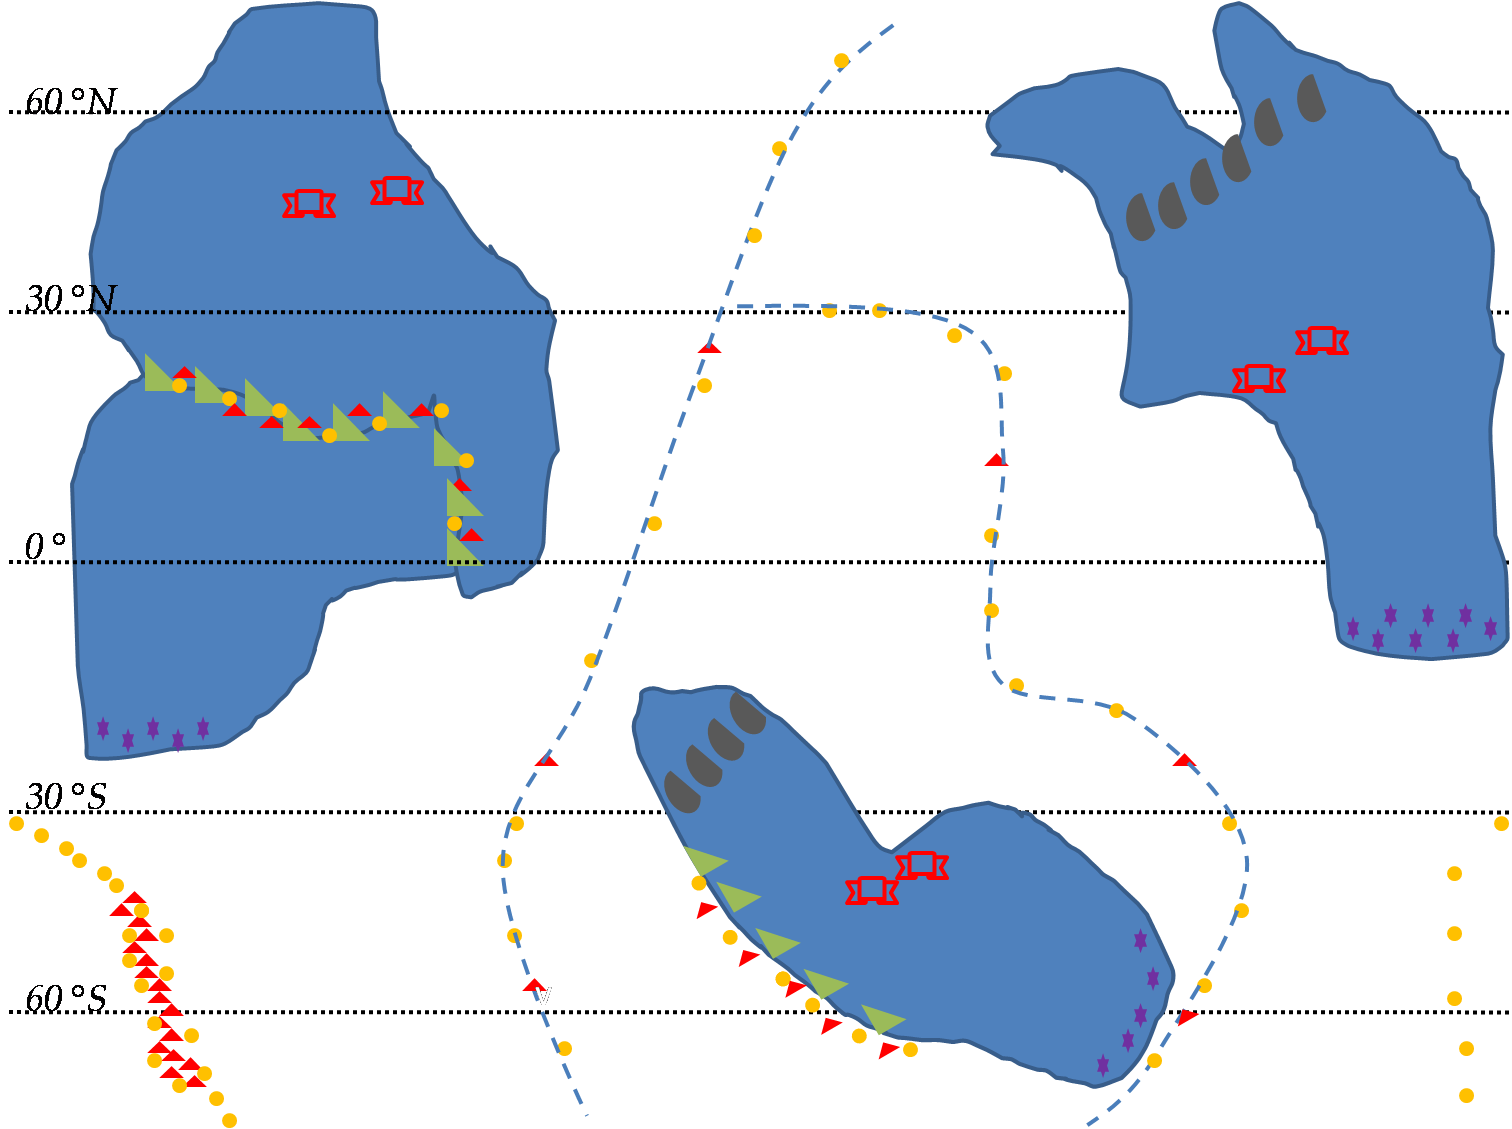
\includegraphics[width=0.95\textwidth]{DerivaContinental}
  \caption{Mapa do Planeta Reverso}
\end{figure}
   \begin{figure}[h!]
  \centering
    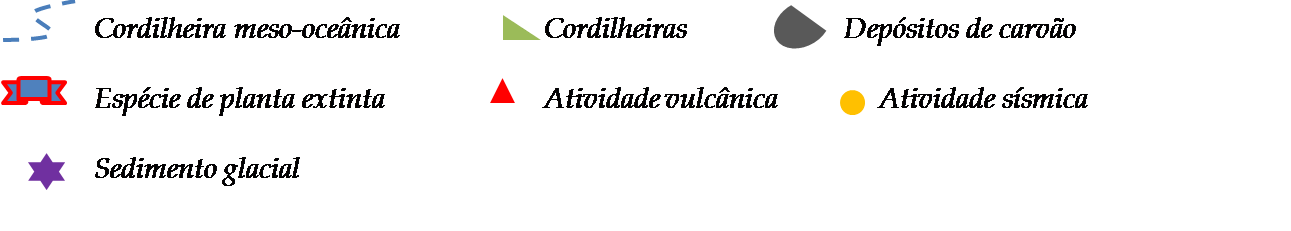
\includegraphics[width=0.95\textwidth]{Legenda}
 \end{figure}
   
  \item[(a)] Identifique na figura quais os tipos de encontros de placas tectônicas presentes. Justifique sua resposta.
  \item[(b)] Identifique os tipos de margens continentais encontradas. Que informações você usou para fazer a identificação?
  \item[(c)] Fossas oceânicas existem em encontros de placas tectônicas e são classificadas em dois grupos. Quais são esses grupos e qual a diferença entre elas?
  \item[(d)] Na figura podem ser observadas algumas evidências que sustentam a teoria da deriva continental? Quais são essas evidências? Explique a teoria da deriva continental. 

  \newpage
  
  \item[2] Faça um desenho esquemático da estratificação vertical de salinidade e temperatura vertical dos oceanos em regiões polares, temperadas e tropicais. Identifique e descreva as características das três camadas. 
  
  \item[3] Explique as mudanças sazonais que ocorrem na termoclina de uma região temperada.
  
  \item[4] Qual a origem dos sedimentos encontrados no ambiente marinho? 
  
  \item[6] Você é o coordenador(a)-científico de uma expedição que tem por objetivo coletar amostras de sedimentos em diferentes regiões do Oceano Atlântico. Entre as suas responsabilidades está a tomada de decisões para a amostragem em função do seu conhecimento oceanográfico.
  \item[(a)] O trabalho requer a coleta de sedimentos carbonáticos na plataforma continental. Qual região do oceano você escolherá para esse tipo de coleta. Lembre que você precisa justificar essa escolha para a sua equipe de trabalho.
  \item[(b)] São necessárias coletas de sedimento em áreas profundas para a identificação de vasas de foraminíferos que serão usadas para datação do material. Qual será o embasamento teórico que você usará para decidir em quais profundidades essas coletas serão realizadas?
  \item[(c)] Um dos objetivos dos trabalhos é avaliar a composição mineralógica das argilas vermelhas. Como você fará a escolha dos locais de coleta para que sejam coletados sedimentos com esse material?
    
  \item[7] Quais os fatores afetam a distribuição horizontal da salinidade nos oceanos? Em função desses fatores como ocorre a distribuição de sal nos oceanos (na camada superficial)?
  
  \item[8] Qual a diferença entre temperatura {\it in-situ} e temperatura potencial? Por que é importante trabalhar com valores de temperatura potencial em oceanografia?
  
  \item[9] Defina densidade potencial. Qual diferença pode ser observada quando trabalhamos com dados de densidade e densidade potencial?
  
  
  \end{itemize}



\end{document}
